\begin{center}
\underline{\Large{T.P.N°6: Uniones soldadas y elementos sometidos a tracción}}
\end{center}

\begin{enumerate}
\item Diseñar la unión soldada viga – columna. La viga es un perfil IPN 200 y la columna está
formada por dos perfiles UPN 180. Tiene una carga aplicada de 40kN con una excentricidad
de 1m como se muestra en la figura. El acero de la perfileria es F-24 y el la resistencia del
material de aporte del electrodo tiene una resistencia mínima a tracción de 480MPa.

\begin{figure}[H]
\begin{center}
     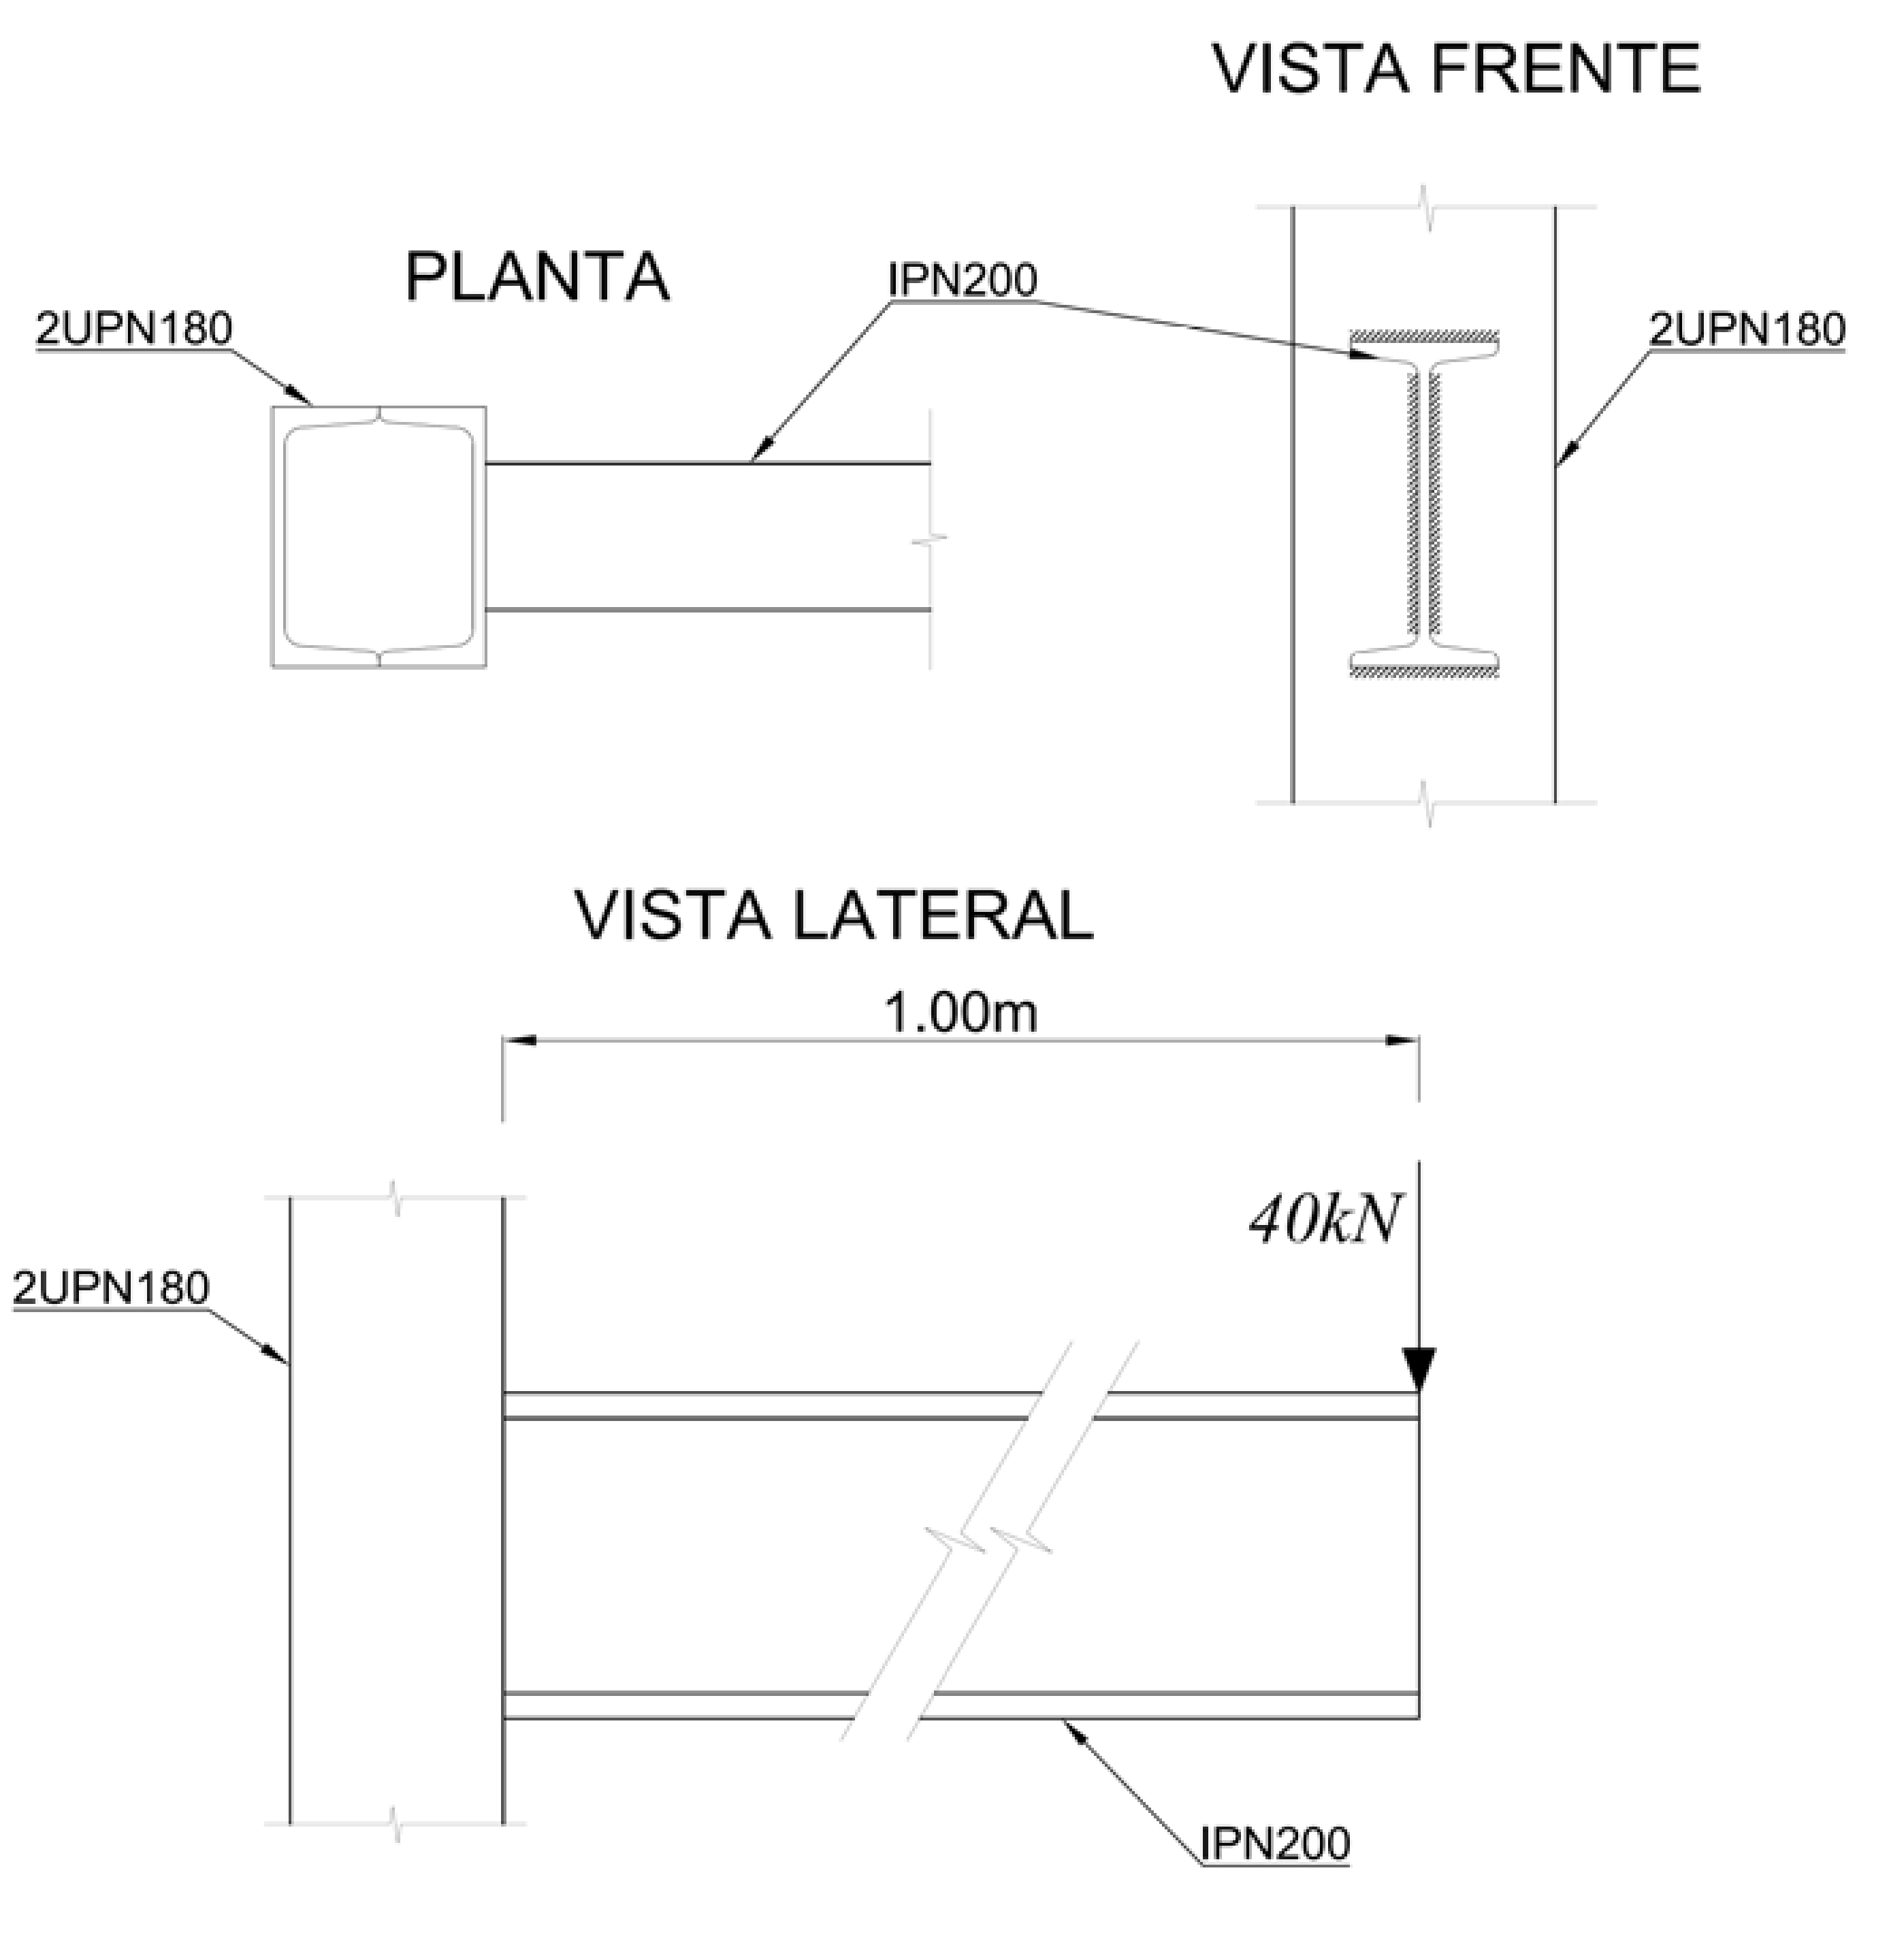
\includegraphics[scale = 1]{chapters/chapter_1/images/figura1.png}
\end{center}
\caption{Unión soldada viga – columna}
\end{figure}
\item Redimensionar la unión del ejercicio 1 del trabajo práctico N° 5, utilizando soldadura. El
material de aporte del electrodo tiene una resistencia mínima a tracción de 480MPa.

\item Verificar la barra a tracción de del ejercicio 1 del trabajo práctico N° 5, tanto para la unión
abulonada, como soldada.

\end{enumerate}

\newpage

\begin{center}
\underline{\Large{Solución}}
\end{center}

\begin{enumerate}
\item Unión soldada viga – columna. La viga es un perfil IPN 200 y la columna está
formada por dos perfiles UPN 180.
\begin{itemize}
\item \underline{Datos}
\begin{align*}
& \text{Acero F-24}\\
& F_u = 370MPa\\
& F_y = 235MPa
\end{align*}

\begin{figure}[H]
\begin{center}
     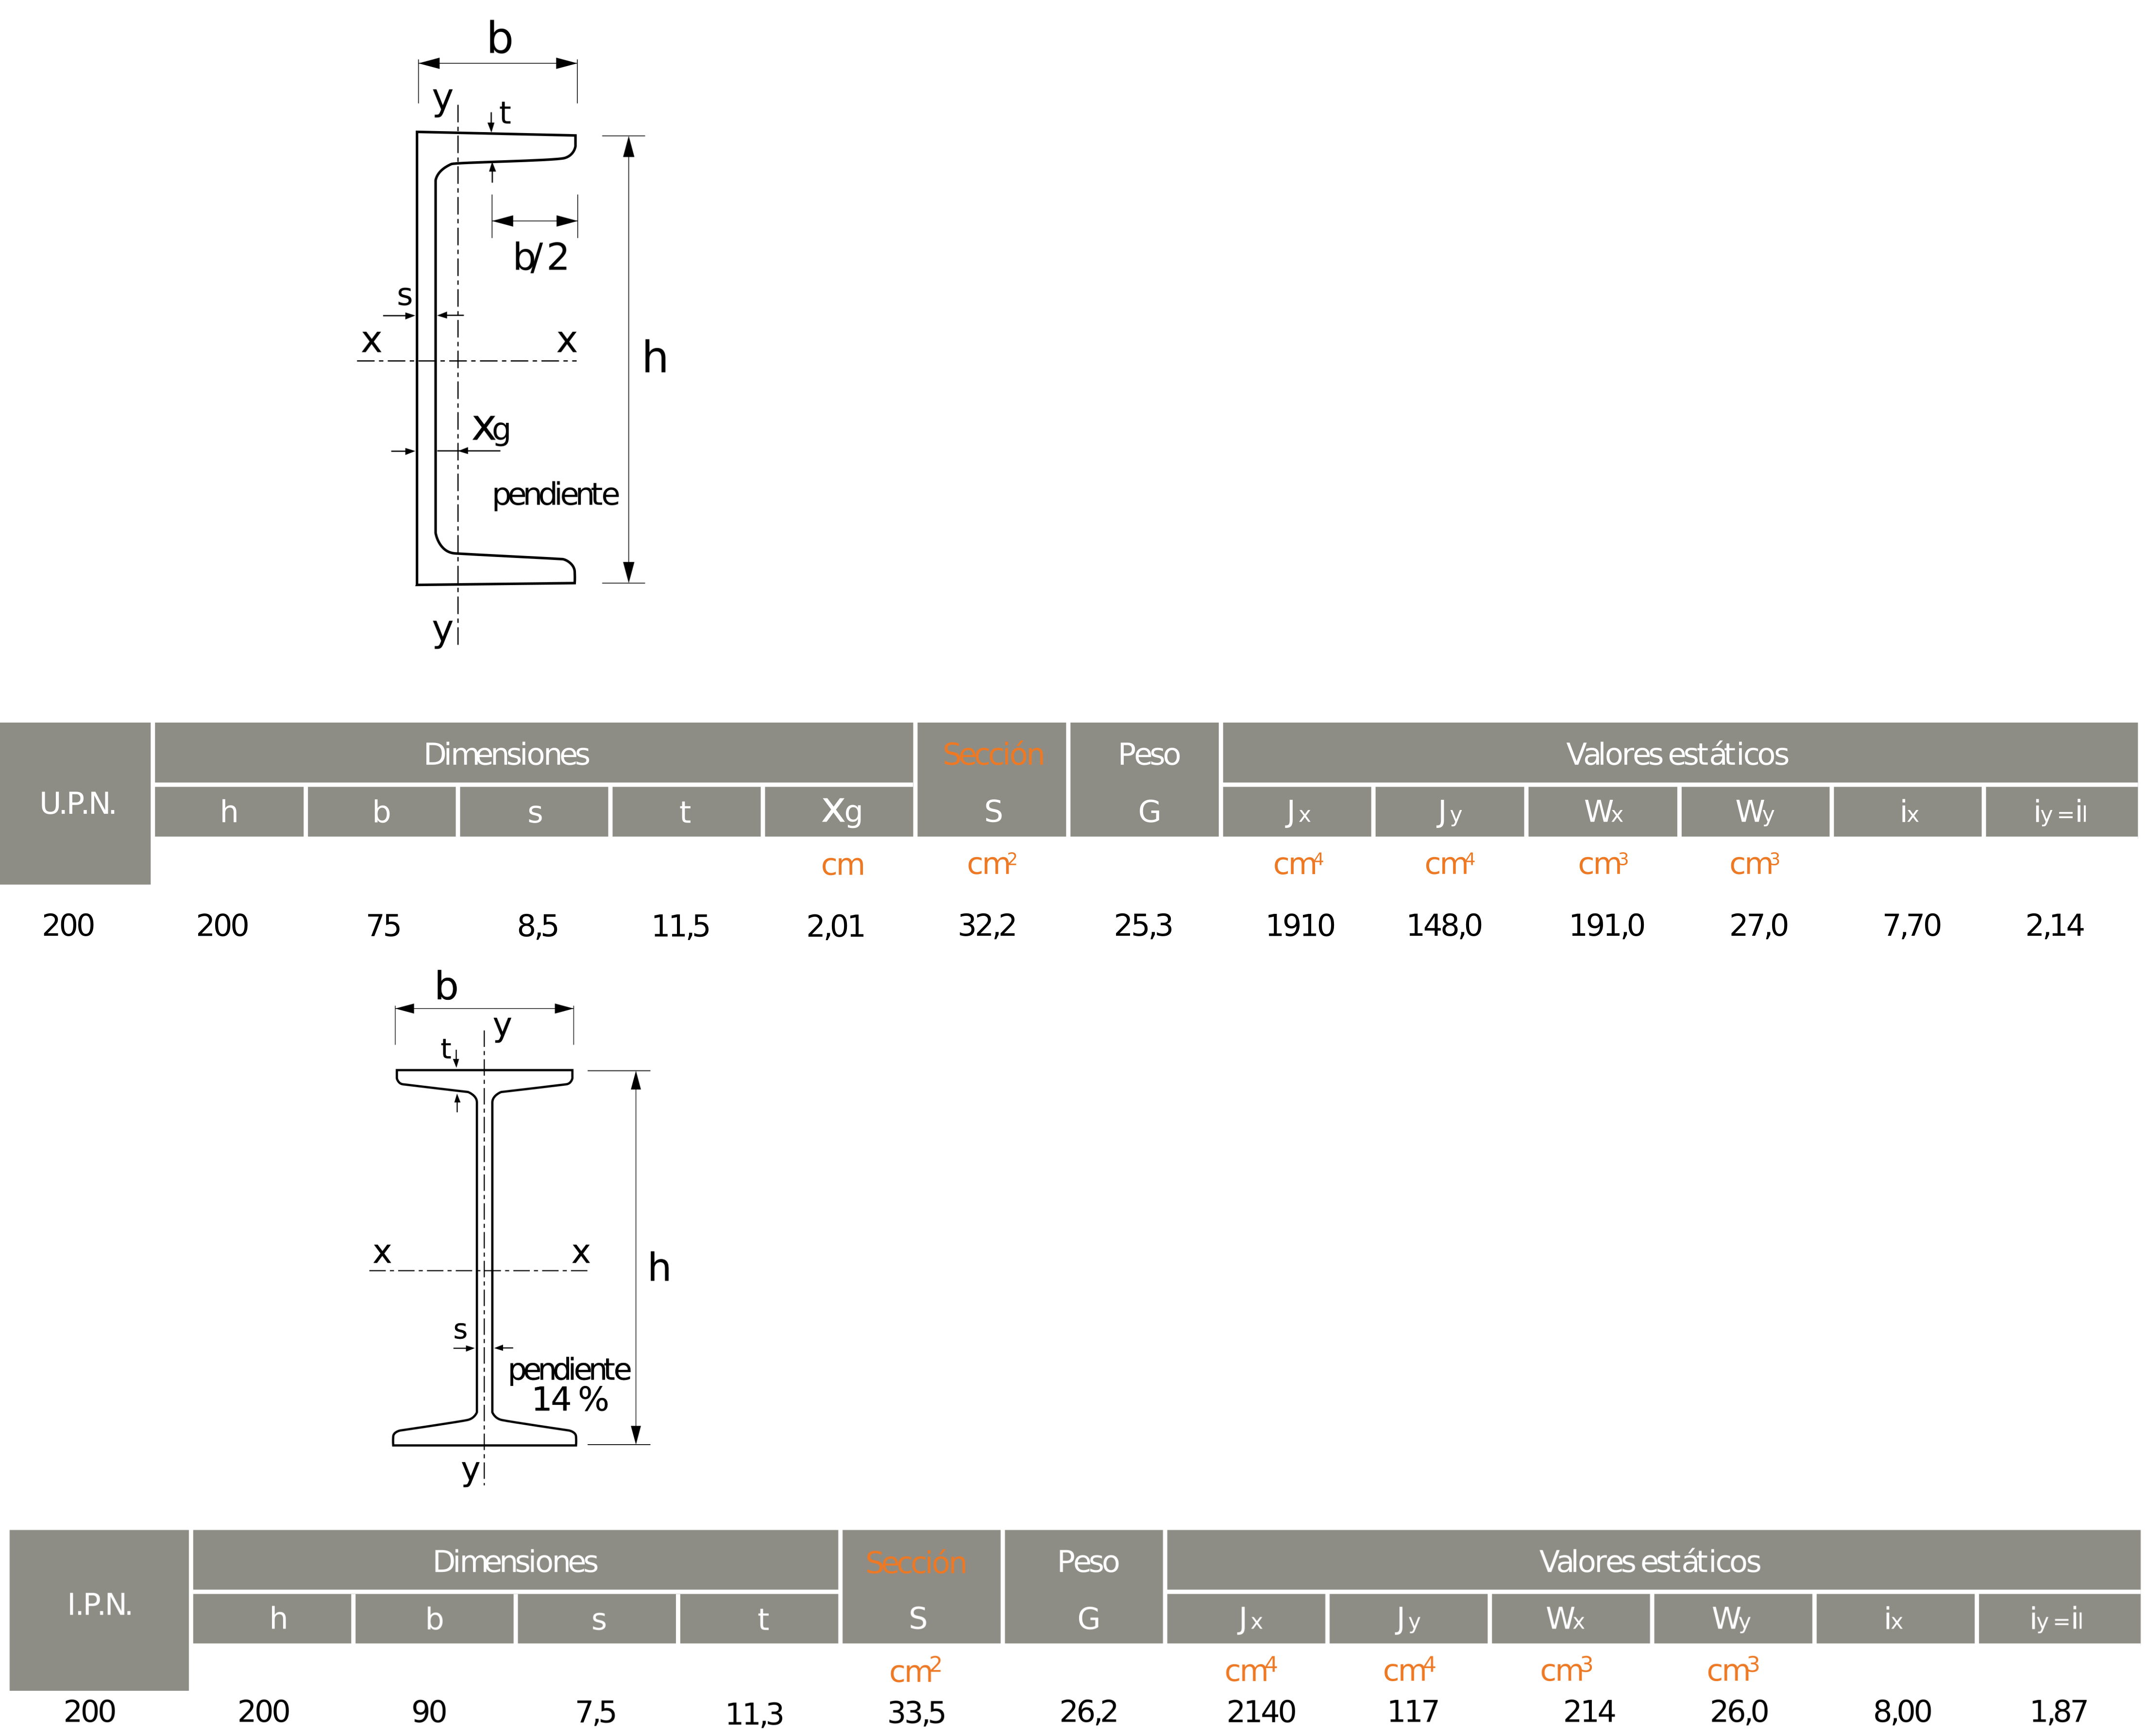
\includegraphics[scale = 0.8]{chapters/chapter_1/images/figura2.png}
\end{center}
\caption{Perfiles IPN200 y UPN180}
\end{figure}

\begin{align*}
& \text{IPN200}\\
& t_1 = 0.75 cm
\end{align*}
\begin{align*}
& \text{UPN180}\\
& t_2 = 0.80 cm
\end{align*}
\begin{align*}
& \text{Electrodo}\\
& F_{exx} = 480MPa\\
\end{align*}

\item \underline{Estado de Cargas}
\begin{align*}
& P = 40KN \\
& M = P \cdot d = 40KN \cdot 100cm = \framebox{$4000 KN \cdot cm$}
\end{align*}

\item \underline{Lados del filete}
\begin{align*}
& W_{min} = 5mm \Rightarrow \text{a partir de los espesores a unir, UPN180 = 8mm, y de la tabla J.2.4}\\
& W_{max} = 8mm - 2mm = 6mm
\end{align*}
Adopto un filete de soldadura con $W = \framebox{$6 mm$}$\\
Los puntos más comprometidos en los cordones de soldaduras son el A, sometido a tracción y corte, y el B, sometido a tracción, debido a la excentricidad de las cargas.\\

\begin{figure}[H]
\begin{center}
     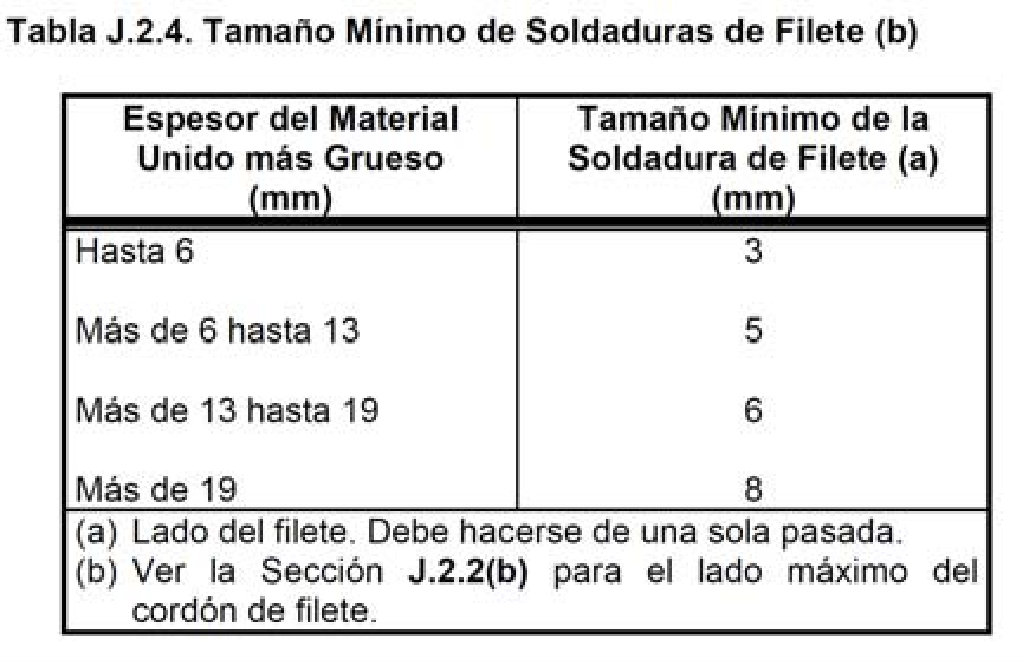
\includegraphics[scale = 1]{chapters/chapter_1/images/tablaJ24.png}
\end{center}
\caption{Tabla J.2.4}
\end{figure}
\begin{figure}[H]
\begin{center}
     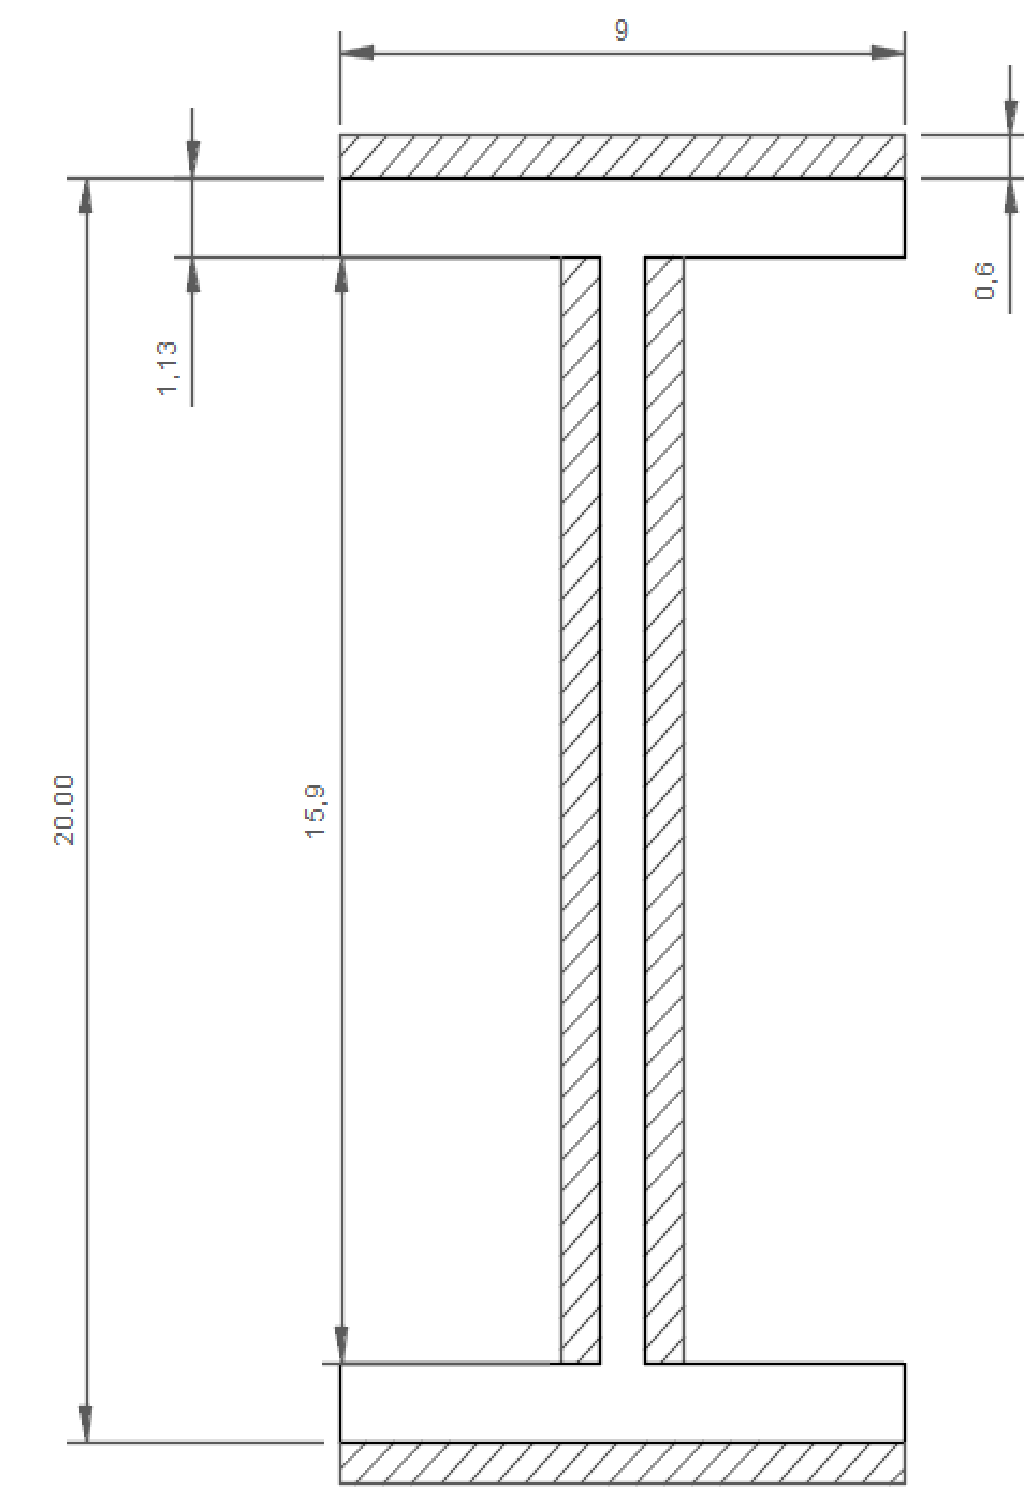
\includegraphics[scale = 0.6]{chapters/chapter_1/images/ipn200.png}
\end{center}
\caption{Perfil IPN200 y filetes de soldadura}
\end{figure}
\begin{figure}[H]
\begin{center}
     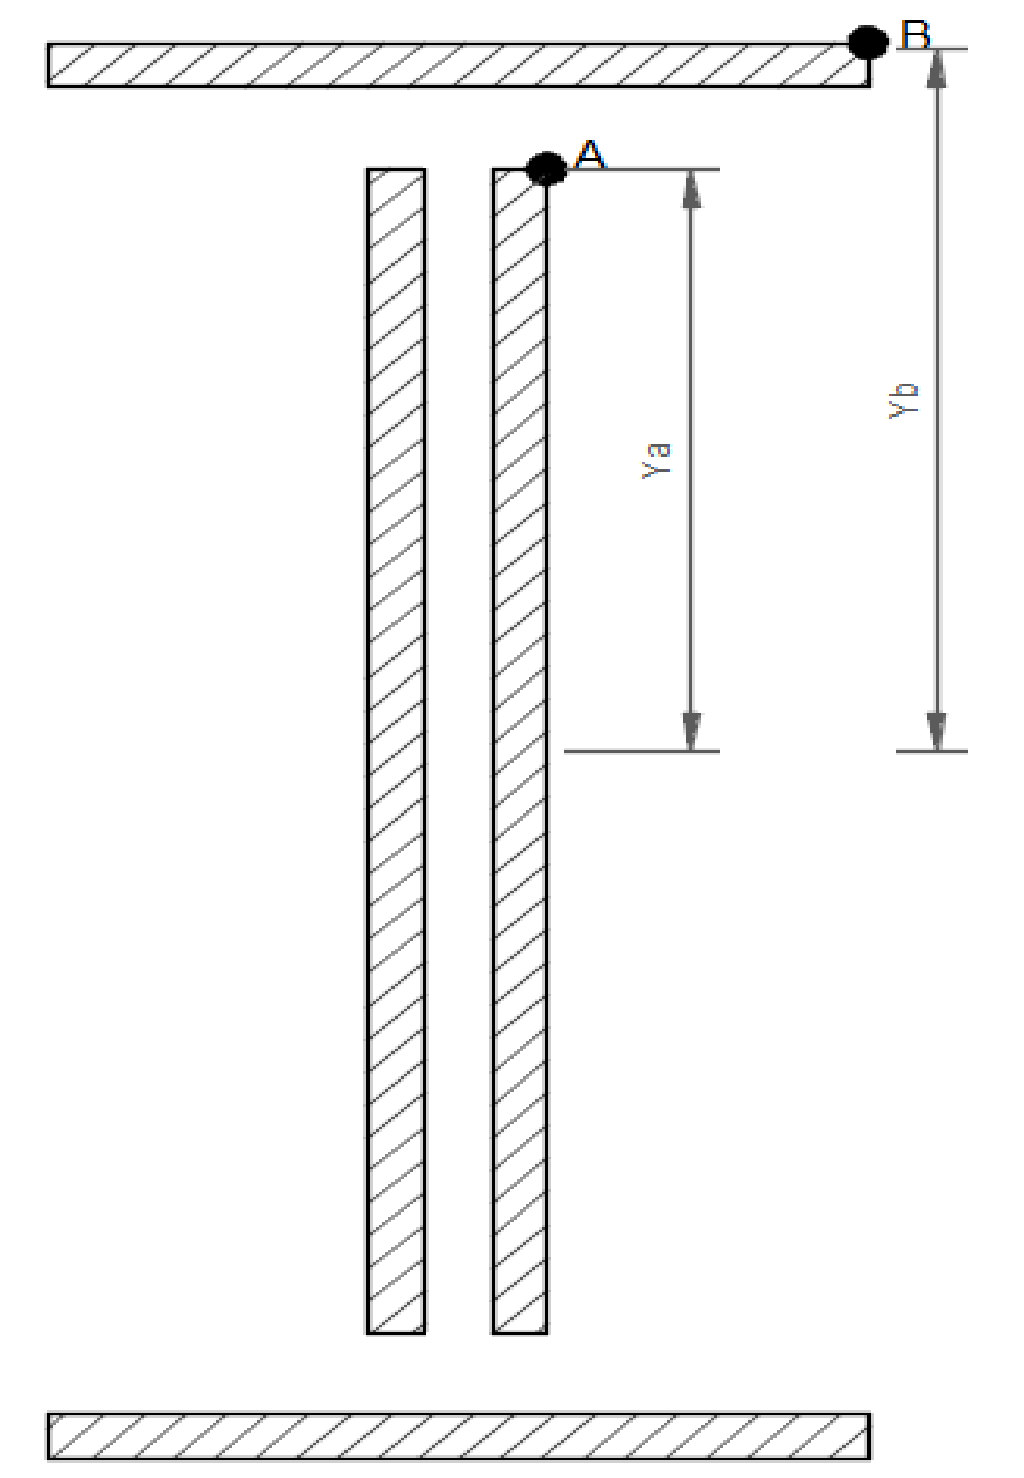
\includegraphics[scale = 0.8]{chapters/chapter_1/images/soldadura.png}
\end{center}
\caption{Filetes de soldadura - Puntos críticos}
\end{figure}

\item \underline{Estudio del Punto A}
\begin{align*}
& L = 2 \cdot 15.9cm = \framebox{$31.8cm$} \\
& A_w = 0.707 \cdot W \cdot L \Rightarrow \text{área efectiva} \\
& A_w = 0.707 \cdot 0.6 cm \cdot 31.8cm = \framebox{$13.48 cm^2$} \\
\end{align*}
Tensiones de corte y tracción en la soldadura.\\
\begin{align*}
& f_v = \frac{P}{A_w \cdot 10^{-1}} = \frac{40KN}{13.48cm^2 \cdot 10^{-1}} = \framebox{$29.65MPa$} \\
& J_{x1} = 2 \cdot \frac{b \cdot h^3}{12} = 2 \cdot \frac{(0.707 \cdot 0.6cm) \cdot (15.9cm)^3}{12} = \framebox{$284.19cm^4$} \\
& J_{x2} = \frac{b \cdot h^3}{12} + A \cdot y^2 \rightarrow \text{Steiner para los cordones horizontales} \\
& J_{x2} = 2 \cdot \Big[\frac{9cm \cdot (0.707 \cdot 0.6cm)^3}{12} + (0.707 \cdot 0.6cm \cdot 9cm) \cdot \Big(10cm+ \frac{0.707 \cdot 0.6cm}{2}\Big)^2\Big] \\
& J_{x2} = \framebox{$796.52cm^4$} \\
& J_x = J_{x1} + J_{x2} = 284.19cm^4 + 796.52cm^4 = \framebox{$1080.71cm^4$} \\
& f_n = \frac{M}{S_w \cdot 10^{-1}} = \frac{M \cdot y_A}{J_x \cdot 10^{-1}} = \frac{4000 KN \cdot cm \cdot \frac{15.9cm}{2}}{1080.71cm^4 \cdot 10^{-1}} = \framebox{$294.25MPa$} \\
& f_c = \sqrt{f_v^2 + f_n^2} = \sqrt{(29.65MPa)^2 + (294.25MPa)^2} = \framebox{$295.74MPa$} \\
& f_{\text{diseño}} = 0.6 \cdot (0.6 \cdot F_{exx}) = 0.6 \cdot (0.6 \cdot 480MPa) = \framebox{$172.8MPa$} \\
& f_c < f_{\text{diseño}} \\
& 295.74MPa < 172.8MPa \Rightarrow \text{No verifica}
\end{align*}
\newpage
\item \underline{Estudio del Punto B}

Tensiones de tracción en la soldadura.\\
\begin{align*}
& J_{x1} = 2 \cdot \frac{b \cdot h^3}{12} = 2 \cdot \frac{(0.707 \cdot 0.6cm) \cdot (15.9cm)^3}{12} = \framebox{$284.19cm^4$} \\
& J_{x2} = \frac{b \cdot h^3}{12} + A \cdot y^2 \rightarrow \text{Steiner para los cordones horizontales} \\
& J_{x2} = 2 \cdot \Big[\frac{9cm \cdot (0.707 \cdot 0.6cm)^3}{12} + (0.707 \cdot 0.6cm \cdot 9cm) \cdot \Big(10cm+ \frac{0.707 \cdot 0.6cm}{2}\Big)^2\Big] \\
& J_{x2} = \framebox{$796.52cm^4$} \\
& J_x = J_{x1} + J_{x2} = 284.19cm^4 + 796.52cm^4 = \framebox{$1080.71cm^4$} \\
& y_B = \frac{h}{2} + 0.707 \cdot W = \frac{20cm}{2} + 0.707 \cdot 0.6cm = \framebox{$10.42cm$} \\
& f_n = \frac{M}{S_w \cdot 10^{-1}} = \frac{M \cdot y_B}{J_x \cdot 10^{-1}} = \frac{4000 KN \cdot cm \cdot 10.42cm}{1080.71cm^4 \cdot 10^{-1}} = \framebox{$385.67MPa$} \\
& f_{\text{diseño}} = 0.6 \cdot (0.6 \cdot F_{exx}) = 0.6 \cdot (0.6 \cdot 480MPa) = \framebox{$172.8MPa$} \\
& f_n < f_{\text{diseño}} \\
& 385.67MPa < 172.8MPa \Rightarrow \text{No verifica}
\end{align*}

Adoptamos un perfil más grande IPN320.\\

\begin{figure}[H]
\begin{center}
     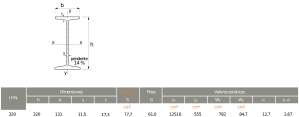
\includegraphics[scale = 0.8]{chapters/chapter_1/images/ipn320_perfil.png}
\end{center}
\caption{Perfil IPN320}
\end{figure}

\begin{figure}[H]
\begin{center}
     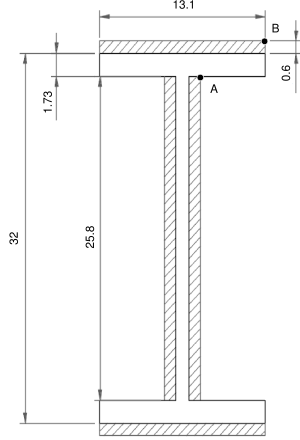
\includegraphics[scale = 0.6]{chapters/chapter_1/images/ipn320.png}
\end{center}
\caption{Perfil IPN320 y filetes de soldadura}
\end{figure}
\item \underline{Estudio del Punto A}
\begin{align*}
& L = 2 \cdot 25.8cm = \framebox{$51.6cm$} \\
& A_w = 0.707 \cdot W \cdot L \Rightarrow \text{área efectiva} \\
& A_w = 0.707 \cdot 0.6 cm \cdot 51.6cm = \framebox{$21.89 cm^2$} \\
\end{align*}
\newpage
Tensiones de corte y tracción en la soldadura.\\
\begin{align*}
& f_v = \frac{P}{A_w \cdot 10^{-1}} = \frac{40KN}{21.89cm^2 \cdot 10^{-1}} = \framebox{$18.27MPa$} \\
& J_{x1} = 2 \cdot \frac{b \cdot h^3}{12} = 2 \cdot \frac{(0.707 \cdot 0.6cm) \cdot (25.8cm)^3}{12} = \framebox{$1214.17cm^4$} \\
& J_{x2} = \frac{b \cdot h^3}{12} + A \cdot y^2 \rightarrow \text{Steiner para los cordones horizontales} \\
& J_{x2} = 2 \cdot \Big[\frac{13.1cm \cdot (0.707 \cdot 0.6cm)^3}{12} + (0.707 \cdot 0.6cm \cdot 13.1cm) \cdot \Big(16cm+ \frac{0.707 \cdot 0.6cm}{2}\Big)^2\Big] \\
& J_{x2} = \framebox{$2921.29cm^4$} \\
& J_x = J_{x1} + J_{x2} = 1214.17cm^4 + 2921.29cm^4 = \framebox{$4135.46cm^4$} \\
& f_n = \frac{M}{S_w \cdot 10^{-1}} = \frac{M \cdot y_A}{J_x \cdot 10^{-1}} = \frac{4000 KN \cdot cm \cdot \frac{25.8cm}{2}}{4135.46cm^4 \cdot 10^{-1}} = \framebox{$124.77MPa$} \\
& f_c = \sqrt{f_v^2 + f_n^2} = \sqrt{(18.27MPa)^2 + (124.77MPa)^2} = \framebox{$126.11MPa$} \\
& f_{\text{diseño}} = 0.6 \cdot (0.6 \cdot F_{exx}) = 0.6 \cdot (0.6 \cdot 480MPa) = \framebox{$172.8MPa$} \\
& f_c < f_{\text{diseño}} \\
& 126.11MPa < 172.8MPa \Rightarrow \text{Verifica}
\end{align*}

\item \underline{Estudio del Punto B}

Tensiones de tracción en la soldadura.\\
\begin{align*}
& J_{x1} = 2 \cdot \frac{b \cdot h^3}{12} = 2 \cdot \frac{(0.707 \cdot 0.6cm) \cdot (25.8cm)^3}{12} = \framebox{$1214.17cm^4$} \\
& J_{x2} = \frac{b \cdot h^3}{12} + A \cdot y^2 \rightarrow \text{Steiner para los cordones horizontales} \\
& J_{x2} = 2 \cdot \Big[\frac{13.1cm \cdot (0.707 \cdot 0.6cm)^3}{12} + (0.707 \cdot 0.6cm \cdot 13.1cm) \cdot \Big(16cm+ \frac{0.707 \cdot 0.6cm}{2}\Big)^2\Big] \\
& J_{x2} = \framebox{$2921.29cm^4$} \\
& J_x = J_{x1} + J_{x2} = 1214.17cm^4 + 2921.29cm^4 = \framebox{$4135.46cm^4$} \\
& y_B = \frac{h}{2} + 0.707 \cdot W = \frac{32cm}{2} + 0.707 \cdot 0.6cm = \framebox{$16.42cm$} \\
& f_n = \frac{M}{S_w \cdot 10^{-1}} = \frac{M \cdot y_B}{J_x \cdot 10^{-1}} = \frac{4000 KN \cdot cm \cdot 16.42cm}{4135.46cm^4 \cdot 10^{-1}} = \framebox{$158.86MPa$} \\
& f_{\text{diseño}} = 0.6 \cdot (0.6 \cdot F_{exx}) = 0.6 \cdot (0.6 \cdot 480MPa) = \framebox{$172.8MPa$} \\
& f_n < f_{\text{diseño}} \\
& 158.86MPa < 172.8MPa \Rightarrow \text{Verifica}
\end{align*}
\end{itemize}
\newpage
\item Redimensionar la unión del ejercicio 1 del TPN° 5.
\begin{itemize}
\item \underline{Datos}
\begin{align*}
& \text{Acero F-24}\\
& F_u = 370MPa\\
& F_y = 235MPa
\end{align*}

\begin{figure}[H]
\begin{center}
     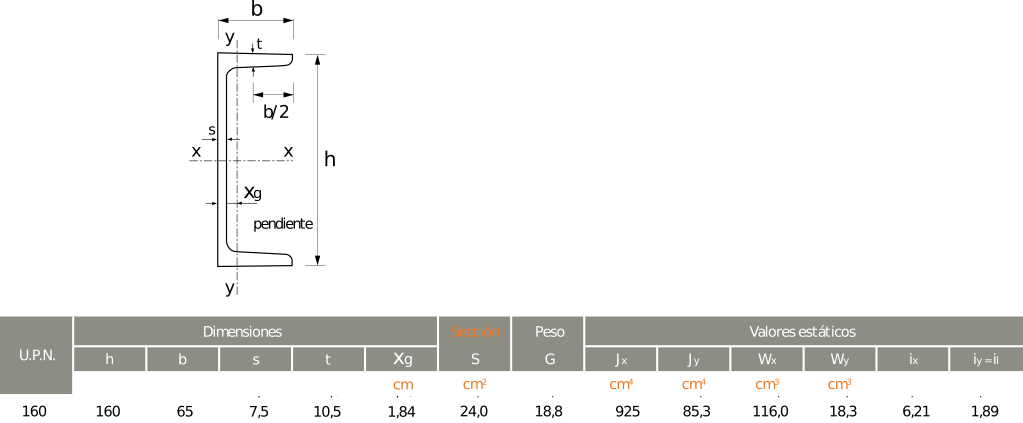
\includegraphics[scale = 0.8]{chapters/chapter_1/images/upn160.png}
\end{center}
\caption{Perfil UPN160}
\end{figure}

\begin{align*}
& \text{Cartela}\\
& t_1 = 0.952 cm
\end{align*}
\begin{align*}
& \text{UPN160}\\
& t_2 = 0.75 cm \\
& A_g = 24 cm^2 \\
& X_g = e_x = 1.84 cm
\end{align*}
\begin{align*}
& \text{Electrodo}\\
& F_{exx} = 480MPa\\
\end{align*}
\newpage
\item \underline{\textbf{Caso 1:}}
Adoptamos filetes longitudinales de igual longitud, no se tiene en cuenta la excentricidad de la carga con respecto al plano de soldadura.\\
\item \underline{Lados del filete}
\begin{align*}
& W_{min} = 5mm \Rightarrow \text{a partir de los espesores a unir, UPN160 = 7.5mm, y de la tabla J.2.4}\\
& W_{max} = 7.5mm - 2mm = 5.5mm
\end{align*}
Adopto un filete de soldadura con $W = \framebox{$5 mm$}$\\

\item \underline{Resistencia de diseño}
\begin{align*}
& R_d = \phi \cdot F_w \cdot A_w \cdot (10)^{-1} \Rightarrow \text{con $\phi = 0.60$ y $F_w = 0.60 \cdot F_{exx}$ de tabla J.2.5}\\
& A_w = W \cdot Cos(45\text{°}) \cdot L = 0.707 \cdot W \cdot L \\
& R_d = 0.60 \cdot (0.60 \cdot F_{exx}) \cdot 0.707 \cdot W \cdot L \cdot (10)^{-1}
\end{align*}

\item \underline{Longitud del cordón de soldadura}
\begin{align*}
& \frac{F_u}{R_d} = 1\\
& \frac{F_u}{0.60 \cdot (0.60 \cdot F_{exx}) \cdot 0.707 \cdot W \cdot L \cdot (10)^{-1}} = 1\\
& \Rightarrow L = \frac{F_u}{0.60 \cdot (0.60 \cdot F_{exx}) \cdot 0.707 \cdot W \cdot (10)^{-1}} \\
& L = \frac{450KN}{0.60 \cdot (0.60 \cdot 480MPa) \cdot 0.707 \cdot 0.5cm \cdot (10)^{-1}} = \framebox{$73.66cm$} \\
& \text{Distribuimos la longitud en dos cordones iguales} \Rightarrow L* = \frac{L}{2} = \frac{73.66cm}{2} = \framebox{$36.83cm$} \\
& \text{Considerando las pérdidas de calidad de soldadura en el inicio y fin del cordón} \\
& \Rightarrow L = L* + 2 \cdot W = 36.83cm + 2 \cdot 0.5cm = \framebox{$37.83cm$} \\
\end{align*}
Adopto una longitud de soldadura $L_1 = \framebox{$38 cm$}$\\
\begin{figure}[H]
\begin{center}
     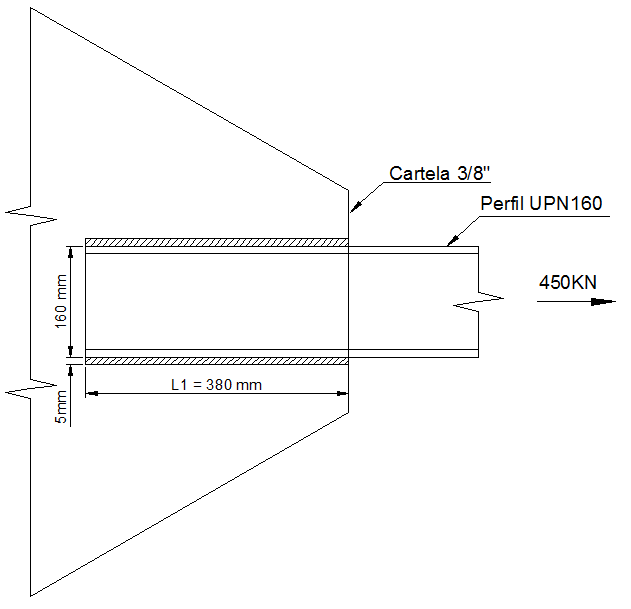
\includegraphics[scale = 0.8]{chapters/chapter_1/images/figura3.png}
\end{center}
\caption{Unión soldada UPN160}
\end{figure}

\item \underline{\textbf{Caso 2:}}
Adoptamos filetes longitudinales de igual longitud y un filete transversal, no se tiene en cuenta la excentricidad de la carga con respecto al plano de soldadura.\\
La longitud total es igual a la del Caso 1°) $L = 73.66cm$ \\

\item \underline{Longitud del cordón de soldadura}
\begin{align*}
& L_{total} = 73.66cm \\
& L_3 = 16cm \text{ ancho del perfil UPN160}\\
& 2 \cdot L_2 = L_{total}-L_3-2 \cdot W \\
& L_2 = \frac{L_{total}-L_3-2 \cdot W}{2} \\
& L_2 = \frac{73.66cm-16cm-2 \cdot 0.5cm}{2} = 29cm \\
& \text{Considerando las pérdidas de calidad de soldadura en el inicio y fin del cordón} \\
& \Rightarrow L_2 = L_2 + 2 \cdot W = 29cm + 2 \cdot 0.5cm = \framebox{$30cm$} \\
\end{align*}
Adopto una longitud de soldadura $L_2 = \framebox{$30 cm$}$\\
\begin{figure}[H]
\begin{center}
     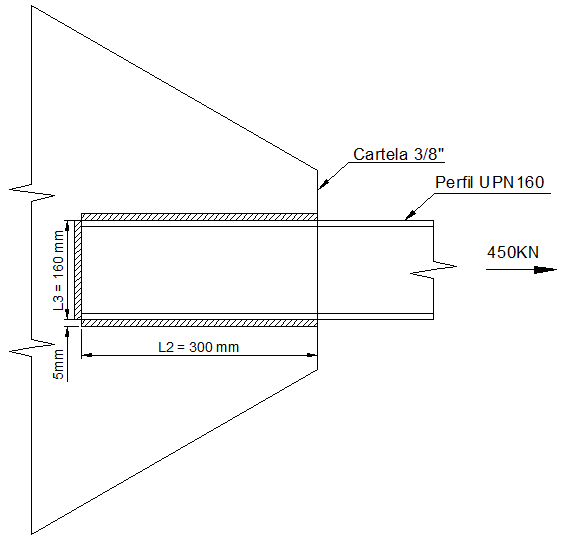
\includegraphics[scale = 0.8]{chapters/chapter_1/images/figura4.png}
\end{center}
\caption{Unión soldada UPN160}
\end{figure}
\newpage
\item \underline{\textbf{Caso 3:}}
Adoptamos filetes longitudinales de igual longitud teniendo en cuenta la flexión que se genera por la excentricidad de la carga con respecto al plano de soldadura.\\

\item \underline{Estado de Cargas}
\begin{align*}
& F_u = 450 KN \\
& e_x = 1.84cm \\
& P_1 = P_2 = F_u \cdot \frac{8cm}{16cm} = 450KN \cdot \frac{8cm}{16cm} = \framebox{$225KN$}\\
& M_1 = M_2 = P_1 \cdot e_x = P_2 \cdot e_x = 225KN \cdot 1.84cm = \framebox{$414 KN \cdot cm$}
\end{align*}

\item \underline{Verificamos las tensiones para los cordones de soldadura}
\begin{align*}
& \text{Cordón 1 = Cordón 2} \\
& \text{Adopto } L = \framebox{$40cm$} \\
& A_w = 0.707 \cdot W \cdot L \Rightarrow \text{área efectiva} \\
& A_w = 0.707 \cdot 0.5 cm \cdot 40cm = \framebox{$14.14 cm^2$} \\
& S_w = \frac{(0.707 \cdot W) \cdot L^2}{6} = \frac{(0.707 \cdot 0.5cm) \cdot (40cm)^2}{6} = \framebox{$94.26 cm^3$} \\
& f_v = \frac{P_1}{A_w \cdot 10^{-1}} = \frac{225KN}{14.14cm^2 \cdot 10^{-1}} = \framebox{$159.12MPa$} \\
& f_n = \frac{M_1}{S_w \cdot 10^{-1}} = \frac{414 KN \cdot cm}{94.26 cm^3 \cdot 10^{-1}} = \framebox{$43.92MPa$} \\
& f_c = \sqrt{f_v^2 + f_n^2} = \sqrt{(159.12MPa)^2 + (43.92MPa)^2} = \framebox{$165.07MPa$} \\
& f_{\text{diseño}} = 0.6 \cdot (0.6 \cdot F_{exx}) = 0.6 \cdot (0.6 \cdot 480MPa) = \framebox{$172.8MPa$} \\
& f_c < f_{\text{diseño}} \\
& 165.07MPa < 172.8MPa \Rightarrow \text{Verifica}
\end{align*}
\begin{figure}[H]
\begin{center}
     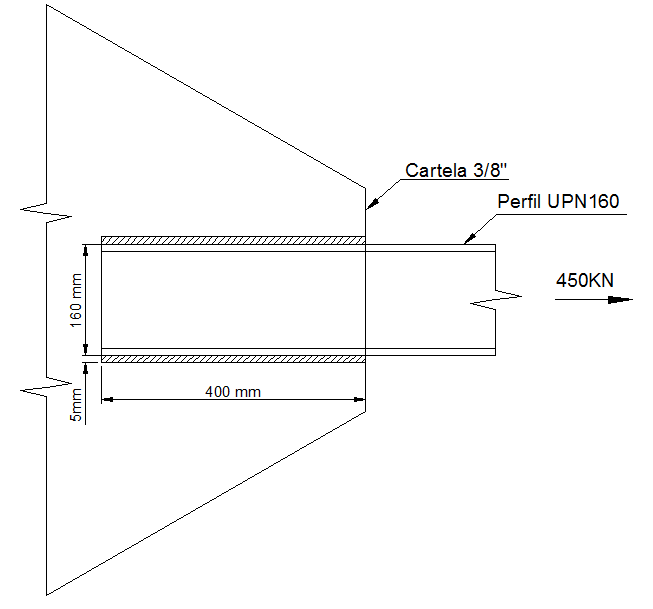
\includegraphics[scale = 0.8]{chapters/chapter_1/images/figura5.png}
\end{center}
\caption{Unión soldada UPN160 con carga excentrica}
\end{figure}
\begin{figure}[H]
\begin{center}
     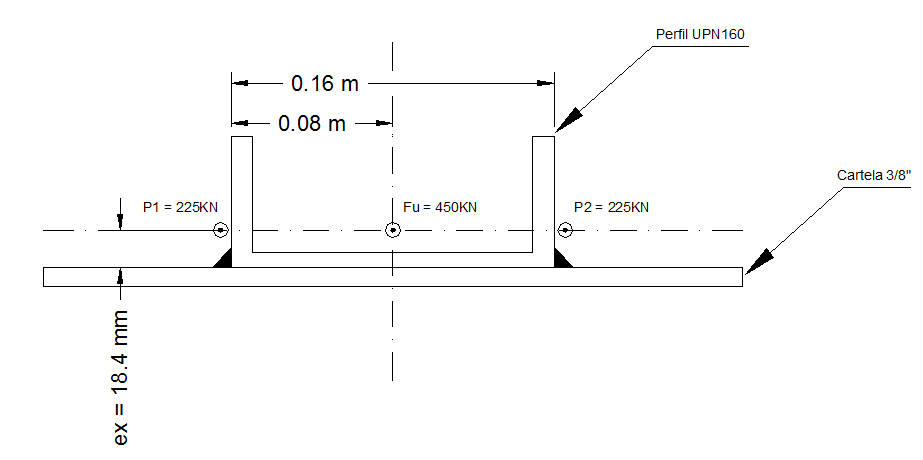
\includegraphics[scale = 0.5]{chapters/chapter_1/images/figura6.png}
\end{center}
\caption{Unión soldada UPN160 con carga excentrica}
\end{figure}
\end{itemize}
\newpage
\item Verificar la barra a tracción del ejercicio 1 del TPN° 5.
\begin{itemize}
\item \underline{\textbf{Verificación para unión abulonada:}}
\begin{figure}[H]
\begin{center}
     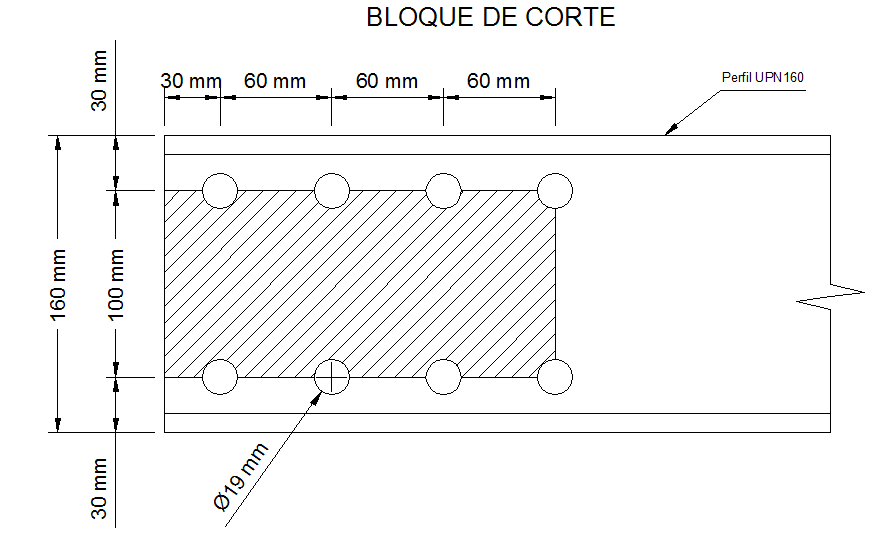
\includegraphics[scale = 0.5]{chapters/chapter_1/images/Bloque_de_Corte_1.png}
\end{center}
\caption{Unión abulonada UPN160}
\end{figure}
La resistencia de diseño de barras traccionadas según el reglamento CIRSOC 301/05, determina $\phi_t \cdot P_n$ como el menor valor obtenido de la consideración de los estados límites de fluencia en la sección bruta, y rotura en la sección neta. Entonces:\\
\item \underline{Para fluencia en la sección bruta:}
\begin{align*}
& \phi_t = 0.90 \\
& P_n = F_y \cdot A_g \cdot 10^{-1} \\
& P_n = 235MPa \cdot 24cm^2 \cdot 10^{-1} = \framebox{$564KN$}\\
& P_u = \phi_t \cdot P_n = 0.90 \cdot 564KN = \framebox{$507.60KN$}
\end{align*}

\item \underline{Para rotura en la sección neta:}
\begin{align*}
& \phi_t = 0.75 \\
& L = 3 \cdot 6cm = 18cm \\
& U = 1 - \frac{x}{L} = 1 - \frac{1.84cm}{18cm} = \framebox{$0.897$}\\
& A_n = A_g - 2 \cdot \text{área de agüjeros} = 24cm^2 - 2 \cdot [0.75cm \cdot (1.90cm + 0.2cm)] = \framebox{$20.85cm^2$}\\
& A_e = U \cdot A_n = 0.897 \cdot 20.85cm^2 = \framebox{$18.70cm^2$}\\
& P_n = F_u \cdot A_e \cdot 10^{-1} \\
& P_n = 370MPa \cdot 18.70cm^2 \cdot 10^{-1} = \framebox{$691.99KN$}\\
& P_u = \phi_t \cdot P_n = 0.75 \cdot 691.99KN = \framebox{$518.99KN$}
\end{align*}
Se adoptara entonces como resistencia de diseño el menor de los valores, en este caso $R_d = \framebox{$507.60KN$}$, como:
\begin{align*}
& P_u = \framebox{$450KN$} \Rightarrow \text{Del trabajo práctico de Uniones abulonadas}\\
& P_u < R_{\text{diseño}} \\
& 450KN < 507.60KN  \Rightarrow \text{Verifica}
\end{align*}

\item \underline{\textbf{Verificación para unión soldada:}}
La resistencia de diseño de barras traccionadas según el reglamento CIRSOC 301/05, determina $\phi_t \cdot P_n$ como el menor valor obtenido de la consideración de los estados límites de fluencia en la sección bruta, y rotura en la sección neta. Entonces:\\
\item \underline{Para fluencia en la sección bruta:}
\begin{align*}
& \phi_t = 0.90 \\
& P_n = F_y \cdot A_g \cdot 10^{-1} \\
& P_n = 235MPa \cdot 24cm^2 \cdot 10^{-1} = \framebox{$564KN$}\\
& P_u = \phi_t \cdot P_n = 0.90 \cdot 564KN = \framebox{$507.60KN$}
\end{align*}

\item \underline{Para rotura en la sección neta:}
\begin{align*}
& \phi_t = 0.75 \\
& U = 1 - \frac{x}{L} = 1 - \frac{1.84cm}{38cm} = \framebox{$0.951$} \\
& A_e = U \cdot A_g = 0.951 \cdot 24cm^2 = \framebox{$22.83cm^2$} \\
& P_n = F_u \cdot A_e \cdot 10^{-1} \\
& P_n = 370MPa \cdot 22.83cm^2 \cdot 10^{-1} = \framebox{$845KN$}\\
& P_u = \phi_t \cdot P_n = 0.75 \cdot 845KN = \framebox{$633.75KN$}
\end{align*}
Se adoptara entonces el menor de los valores, en este caso $P_u = \framebox{$507.60KN$}$, como:
\begin{align*}
& R_d = 0.60 \cdot (0.60 \cdot F_{exx}) \cdot 0.707 \cdot W \cdot L \cdot (10)^{-1} \\
& R_d = 2 \cdot [0.60 \cdot (0.60 \cdot 480MPa) \cdot 0.707 \cdot 0.5cm \cdot 45cm \cdot (10)^{-1}] = \framebox{$549.76KN$}\\
& P_u < R_{\text{diseño}} \\
& 507.60KN < 549.76KN \Rightarrow \text{Verifica}
\end{align*}

\end{itemize}
\end{enumerate}